\documentclass[useAMS,usenatbib, a4paper]{mn2e} \usepackage{natbib} 
\addtolength{\voffset}{-0.5in}
\usepackage{graphicx} \usepackage{amssymb}
\usepackage{amsmath}

\input{macros.tex}

% -----------------------------------------------------------------------------

\title[Time Delays with Gaussian Processes]
{Inference of Gravitational Lens Time Delays Using Gaussian Processes} 
\author[B. J. Brewer]{Brendon J. Brewer$^1$, Philip J. Marshall$^2$, Gregory Dobler$^3$ \\
$^1$Department of Physics, University of California, Santa Barbara, CA, USA \\
$^2$Department of Physics, University of Oxford, Keble Road, Oxford, OX1 3RH, UK \\
$^3$KITP}

\begin{document} 

\date{\today} 
\pagerange{\pageref{firstpage}--\pageref{lastpage}} \pubyear{2011} 
\maketitle \label{firstpage}

% -----------------------------------------------------------------------------

\begin{abstract}

Observations of gravitationally lensed quasars provide a unique method for
measuring cosmological parameters, particularly the Hubble constant $H_0$.
A key part of
this process is the extraction of the time delays from the photometric
monitoring data of the multiple images of the quasar. Quantifying the
uncertainty in this process is challenging, particularly when the time delays
are obscured by the presence of microlensing in the light curves. We present a
fully probabilistic model for the process of inferring the time delays from
the light curve data. In this model, the probability distribution over light
curves is described by a Gaussian Process (GP) whose covariance function
depends on the time delays as well as the properties of the microlensing.
Inferring the parameters of the covariance function from data yields
the time delays, while allowing for a wide range of intrinsic, microlensing, and 
noise-related variability. We test this method extensively on simulated data, 
and find the inferences (including parameter uncertainties) to be robust.
We apply our method to radio and optical monitoring data of the well
studied lenses B1608+656 and RXJ1131$-$123, deriving new time delay estimates complete 
with covariances. The effect on the $H_0$ precision from B1608 is ...

\end{abstract}

\begin{keywords} gravitational lensing --- methods: statistical --- 
\end{keywords}

% -----------------------------------------------------------------------------

\section{Introduction} 

Gravitational lensing has long been recognised as a unique tool for measuring
the cosmological parameters \citep{schechter}. The method makes use of the
intrinsic time variability of a quasar that happens to be multiply imaged. As
the quasar's luminosity varies, each of the multiple images presents the same
fluctuations, but with a time delay $\tau$ that depends on the cosmological
parameters. Therefore, measuring the time delays between the images and
comparing them to those predicted from a model of the gravitational lens
potential allows the cosmological parameters to be estimated.

Historical estimates and problems

The promise of this technique has led to dedicated monitoring programs such as
COSMOGrail \citep[][]{2005A&A...436...25E, 2008A&A...488..481V}. Recently,
thorough investigation of systematic effects and robust lens modelling
techniques have allowed $H_0$ to be measured to a precision of X \% using a
single gravitational lens system \citep{2010ApJ...711..201S}. Specific
systematic effects that were robustly modelled include the uncertainty in the
lens potential reconstruction \citep{2009ApJ...691..277S} and the effects of
external convergence from matter along the line of sight
\citep{2006ApJ...642...30F, 2010ApJ...711..201S}. With large numbers of
suitable gravitational lens systems expected to be found in upcoming surveys
\citep{2010MNRAS.405.2579O}, combining the constraints from many systems can
be expected to yield high precision cosmological measurements
\citep{2010ApJ...712.1378P}, provided sources of systematic error are
understood and well modelled.

However, any inference of $H_0$ from the gravitational lensing method inherits
the uncertainty from the measurements of the time delays themselves. A
thorough investigation of all known sources of uncertainty is an integral part
of measuring cosmological parameters, and thus the purpose of this paper is to
develop and present a reliable method for estimating the uncertainty on the
values of the time delays themselves. The method is Bayesian
\citep{2004kats.book.....O} so the results obtained are probability
distributions for the time delays, and the uncertainties in the time delays
are indicated by the widths of these probability distributions. To describe
the underlying time variation of the quasar and the effects of microlensing on
the light curves, we use Gaussian Processes (GPs), a family of probability
distributions over function space that has computationally convenient
properties \citep{rasmussen}.

Our method for extracting time delays from light curve data is similar in
principle to that presented by \citet{2008ApJ...676...80M}, who described the
effect of microlensing by using simulated microlensing light curves. However,
in practical applications their method becomes computationally prohibitive at
a faster rate than the Gaussian Process approach, because the probability of
finding simulated microlensing tracks that match the observed data decreases
approximately exponentially as the length of the data set grows. In contrast,
GP calculations tend to scale as $O(N^3)$, although this can be improved with
the use of approximations such as conjugate gradient techniques
\citep{gibbsmackay}.

Our method is also related to the curve-shifting approach of
\citet{1996A&A...305...97P}, which aims to find those time delays that
minimise the scatter in the shifted light curves. The primary differences
between the GP approach and standard curve shifting are that the GP approach
is fully Bayesian and allows for exploration of the time delay parameter
space, rather than providing a point estimate. Secondly, it is the likelihood
function, rather than the scatter, which guides the inference, making it clear
how uncertainties are to be obtained. 

An introduction to Gaussian Processes and their applications can be found in
\citet{rasmussen}. however, in their applications, GPs are usually used as a
prior distribution over the space of functions. Here, GPs describe the
sampling distributions, or the probability of the data given the model
parameters. This is a common situation in astrophysics in fields where the
signals can be modelled by a stochastic process, for example quasar
variability \citep{2009ApJ...698..895K, 2010ApJ...721.1014M, 2011ApJ...735...80Z} and solar-like
oscillations of stars \citep{2009MNRAS.395.2226B}.

% -----------------------------------------------------------------------------


\section{The Model}

We begin by defining our model for the prior knowledge about how the time
delays give rise rise to the observed data. This results in a probability
distribution for the data given some unknown parameters, i.e. sampling
distributions $p(D|\theta)$. Once specific data is in hand, the sampling
distributions become a likelihood function for the parameters which can be
combined with a prior distribution $p(\theta)$ to give inferences. By Bayes'
rule, the posterior distribution for some parameters $\theta$ given data $D$
is given by:
\begin{equation}
p(\theta|D = D^*) \propto p(\theta)p(D|\theta)|_{D = D^*}
\end{equation}
where $D^*$ is the actual data set that was observed. Throughout this paper,
the data $D$ are a set of measured magnitudes of multiple images of a QSO; see
Figure~\ref{simdata} for an example data set.

The intrinsic quasar variability, in magnitudes, and in whatever band the
observations are carried out in, is described by a function $f(t)$. For a
four-image system, the resulting light curves, if observed without gaps and
noise, would be described by the functions
\begin{eqnarray}
y_1(t) &=& m_1 + f(t) + \mu_1(t) \\
y_2(t) &=& m_2 + f(t - \tau_2) + \mu_2(t) \\
y_3(t) &=& m_3 + f(t - \tau_3) + \mu_3(t) \\
y_4(t) &=& m_4 + f(t - \tau_4) + \mu_4(t) 
\end{eqnarray}
where $\{m_1, m_2, m_3, m_4\}$ are the mean magnitudes of the images,
$\{\tau_2, \tau_3, \tau_4\}$ are the time delays relative to image 1, and the
functions $\{\mu_1(t), \mu_2(t), \mu_3(t), \mu_4(t)\}$ describe the perturbing
effects of microlensing on each of the light curves. The data then consist of
noisy, irregularly sampled measurements of the light curves $\{y_1(t), y_2(t),
y_3(t), y_4(t)\}$.

{\bf GAUSSIAN ERRORS ON MAGNITUDES?}

{\bf IMPORTANCE OF MEAN MAGS FOR MILLILENSING, CORRELATION WITH MICROLENSING AND INTRINSIC AGN TIMESCALE, NEED FOR INFORMATIVE PRIORS}

We assume that the covariance function for the quasar variability is given by
\begin{eqnarray}
\textnormal{Cov}\left[f(t_1), f(t_2)\right] = C(|t_2 - t_1|)
\end{eqnarray}
where
\begin{eqnarray}
C(\Delta t) = \sigma_{\rm QSO}^2\exp\left(-\frac{\Delta t}{L_{\rm QSO}}\right)
\end{eqnarray}

{\bf COMMENT ON KELLY}

Similarly, the covariance function for each of the microlensing components is
\begin{eqnarray}
\textnormal{Cov}\left[\mu(t_1), \mu(t_2)\right] = C_{\rm micro}(|t_2 - t_1|)
\end{eqnarray}
where
\begin{eqnarray}
C_{\rm micro}(\Delta t) = \sigma_{\rm micro}^2\exp\left(-\left(\frac{\Delta t}{L_{\rm micro}}\right)^{\alpha_{\rm micro}}\right)
\end{eqnarray}

There is a $\sigma_{\rm micro}$  parameter and an $L_{\rm micro}$ parameter
for each image; this is because the stellar density and lens convergence is
different at each image position. In contrast, we use a single $\alpha_{\rm
micro}$   parameter for all images; this is because it is suspected that the
smoothness of the microlensing variations, which $\alpha$ describes, depends
primarily on the size of the microlensed source, and all images are of the
same source. 

The covariance function of the noise-free light curves is then:
\begin{eqnarray}
& & \textnormal{Cov}\left[y_i(t_1), y_j(t_2)\right] \nonumber\\
&=& \left<y_i(t_1)y_j(t_2)\right> \\
&=& \left<\left[f(t_1 - \tau_i) + \mu_i(t_1)\right]\left[f(t_2 - \tau_j) + \mu_j(t_2)\right]\right> \\
&=& \left<f(t_1 - \tau_i)f(t_2 - \tau_j)\right> + \left<\mu_i(t_1)\mu_j(t_2)\right> \\
&=& C_{\rm QSO}(t_1 - \tau_i - t_2 + \tau_j) + \delta_{ij}C_{\rm micro}(t_1 - t_2)
\end{eqnarray}
where the intrinsic variations have been assumed to be uncorrelated with the
microlensing contributions.

The probability distribution for the observed data $\mathbf{y}$ given the
model parameters $\boldsymbol{\theta}$ is a multivariate Gaussian:
\begin{equation}
p(\mathbf{y} | \theta) = \frac{1}{\sqrt{(2\pi)^n \det \mathbf{C}}} \exp\left[-\frac{1}{2}(\mathbf{y} - \mathbf{m})^T\mathbf{C}^{-1}(\mathbf{y} - \mathbf{m})\right]
\end{equation}
where $\mathbf{m}$ is the vector of mean values, and $\mathbf{C}$ is the
covariance matrix of the data, formed by evaluating the covariance function of
the GP at the times of the observations, and then adding diagonal components
to describe the observational errors. That is to say, 

\begin{equation}
\mathbf{C} = \textnormal{Cov}\left[y_i(t_1), y_j(t_2)\right] + \mathbf{C}_{\rm noise}.
\end{equation}
{\bf TODO: WRITE THIS PROPERLY}

Note that in this formalism we are using a  GP to describe the {\it
uncertainty} about the microlensing contributions to the light curves so that
we can model the data. This is not quite the same as asserting that the
microlensing magnifications were generated by a Gaussian Process; it is a way
of accoutning for microlensing fluctuations when inferring the time delays. It
is also the case that {\it other} sources of light curve fluctuation, such as
outliers caused by single epoch calibration errors, will be absorbed by the
``microlensing'' process -- the robustness of the time delay inference in that
situation is something we test in Section~\ref{simdata}. It would be more
realistic, yet much more computationally demanding, to use actual simulated
microlensing  light curves \citep{1999JCoAM.109..353W, 2008ApJ...676...80M,
2010NewA...15..181G}. However, for large source sizes or far from caustic
crossing events, we might expect that the GP approximation is adequate. In
Section~\ref{simdata} we test the model on simulated data containing realistic
microlensing effects, and demonstrate that the time delays are still reliably
inferred despite the GP assumption.

A common situation in astronomy is that final data products, such as light
curves, are returned, with error bars, from a pipeline. However, such error
bars are not always trustworthy, as they may have been underestimated due to
modelling assumptions and approximations in the pipeline. In the context of
light curve modelling, underestimated error bars can be detected if the
scatter in the light curve is better modelled by independent Gaussian noise
than it is by a time-correlated microlensing term. Thus, to improve the
robustness of our method, we include a ``noise boost'' parameter $\kappa$
describing the factor by which the reported error bars should be multiplied.
This is another testable mechanism for accounting for outliers.

In summary, the parameter vector is
\begin{equation}
\left\{ \{\tau\}, \{m\}, \sigma_{\rm QSO}, L_{\rm QSO}, \{\sigma_{\rm micro}\}, \{L_{\rm micro}\}, \alpha_{\rm micro}, \kappa \right\}
\end{equation}
where parameters in braces denote a set (one for each QSO image).  For a
double image lens, the total number of parameters in the model is~12. For a
quad, this number is~20. {\bf CHECK.}  A set of uninformative prior
distributions for these parameters are listed in Table~\ref{priors}; we assign
these priors in the analysis described in the first part of this paper. Later,
we will show how a more informative set of priors can be derived, and used to
improve the precision of the time delay inferences {\bf (WE HOPE)}.

%%%%%%%%%%%%%%%%%%%%%%%%%%%%%%%%%%%%%%%%%%
\begin{table}
\begin{center}
\begin{tabular}{ccc}
Parameter & \vline & Prior \\
\hline
$\tau$ & \vline & $U(-\Delta t/2, \Delta t/2)$ \\ 
$m$ & \vline & $U(y_{\rm min}, y_{\rm max})$ \\
$\sigma_{\rm QSO}$ & \vline & $LU(10^{-3}, 10)$ \\
$L_{\rm QSO}$ & \vline & $LU(10^{-3}\Delta t, 10\Delta t)$ \\
$\sigma_{\rm micro}$ & \vline & $LU(10^{-3}, 10)$ \\
$L_{\rm micro}$ & \vline & $LU(10^{-3}\Delta t, 10\Delta t)$ \\
$\alpha_{\rm micro}$ & \vline & $U(1, 2)$ \\
$\kappa$ & \vline & $LU(1, 10)$
\end{tabular}
\end{center}
\caption{Prior probability distributions for the parameters. $U(a, b)$ denotes
a uniform prior between $a$ and $b$, and $LU(a, b)$ denotes a log-uniform
(that is, uniform in the logarithm of the parameter) prior $\propto 1/x$
between $a$ and $b$. $\Delta t$ is the duration of the data set. All priors
are independent.\label{priors}}
\end{table}
%%%%%%%%%%%%%%%%%%%%%%%%%%%%%%%%%%%%%%%%%%


\subsection{Computational Details}

We use Diffusive Nested Sampling \citep{dnest} to explore the posterior
distribution for the parameters. Metropolis-Hastings updates are used for all
parameters. For those that do not affect the covariance matrix (the $m$'s),
the Cholesky decomposition is not recomputed, making these steps fast. {\bf
DESCRIBE CONSTRUCTION OF CHOLESKY DECOMP AND MOTIVATION - CITE KOSLOWSKI,
R\&W}


% -----------------------------------------------------------------------------

\section{Tests on Simulated Data}\label{simdata}

In this section, we demonstrate the method on simulated data. We first show
that, in the absence of microlensing, we can recover the input time delays and
GP parameters of the intrinsic AGN lightcurve. We then go on to test the
method on the same mock lens systems, but now with plausible microlensing
fluctuations added. These data violate the modelling assumptions, particularly
that of the probability distribution for the microlensing variations being a
GP. 

% - - - - - - - - - - - - - - - - - - - - - - - - - - - - - - - - - - - - - - - 

\subsection{A Sample of Mock Lenses}

Motivated by the need to accurately measure time delays for lens cosmography
in the multi-filter optical imaging survey era, we  we selected three
quadruply-imaged quasar lens systems from the mock LSST  catalog provided by
\citet[][hereafter OM10]{OM10}.\footnote{The catalog is available from
\texttt{http://kipac.stanford.edu/collab/research/lensing}} 

The OM10 mock lenses are designed to represent massive elliptical galaxies;
they have singular isothermal mass distributions, with velocity dispersions
$\vdisp$ drawn from the SDSS velocity function \citep[extrapolated to higher
redshifts assuming no evolution, as in][]{Ogu++08}. The sources were drawn
from a model quasar luminosity function that matches the observed bright and
faint ends. External shears, drawn from a plausible distribution, were
applied. The mock catalog is the product of performing the lens abundance
calculation for the LSST survey by Monte Carlo integration; OM10 found some
3000 well-measured lens systems to be detectable at LSST single-epoch depth
and image quality. Here we consider a typical slice through this sample: from
the 22 systems lying between $0.4 < \zd < 0.6$, $1.6 < \zs < 2.4$ and $150 <
\vdisp < 300$\kms, three were chosen as being representative of the possible
image configurations while also being particularly prone to microlensing
effects: 6 out of the 12 images lie within the lens galaxy effective radius. 

%%%%%%%%%%%%%%%%%%%%%%%%%%%%%%%%%%%%%%%%%%%%
\begin{figure*}
\begin{minipage}{0.32\linewidth}
\centering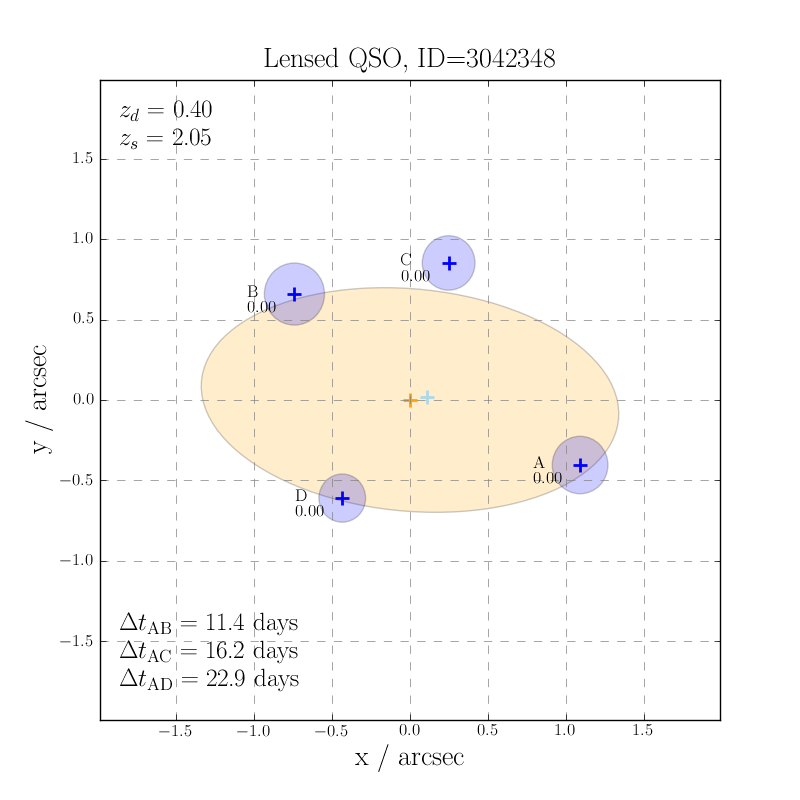
\includegraphics[width=\linewidth]{figs1/oguri_qso_ID=3042348.eps}
\end{minipage}
\begin{minipage}{0.32\linewidth}
\centering\includegraphics[width=\linewidth]{figs1/oguri_qso_ID=3424637.eps}
\end{minipage}
\begin{minipage}{0.32\linewidth}
\centering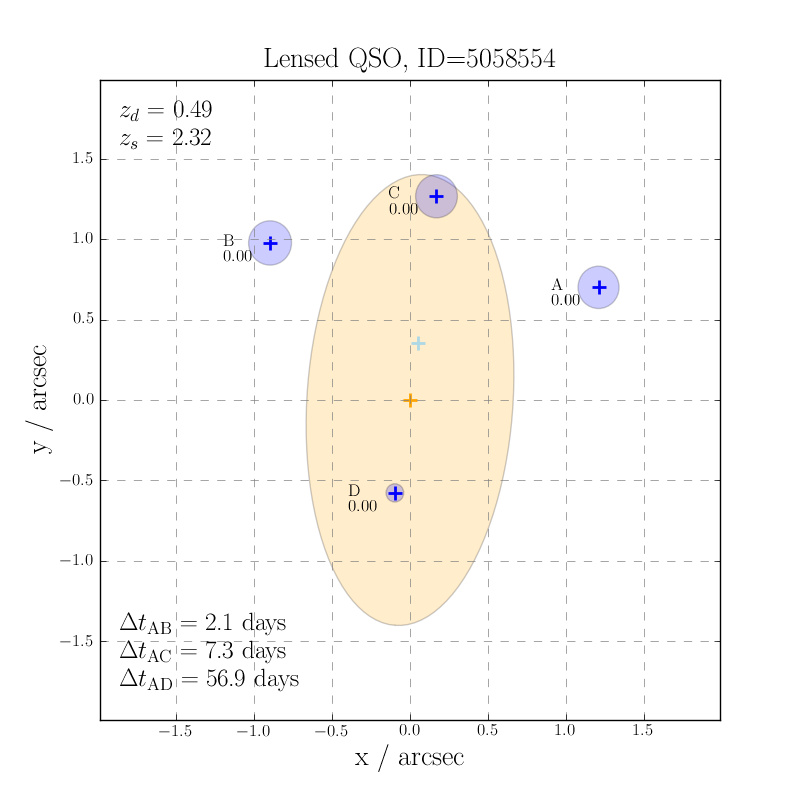
\includegraphics[width=\linewidth]{figs1/oguri_qso_ID=5058554.eps}
\end{minipage}\hfill
\caption{The three simulated lenses, showing image positions (blue) relative
to the lens light effective area (orange). The fraction of surface mass
density in stars ($f^{*}$) at each image position is shown under each image's\label{lenslayouts}}
\end{figure*}
%%%%%%%%%%%%%%%%%%%%%%%%%%%%%%%%%%%%%%%%%%%%


% - - - - - - - - - - - - - - - - - - - - - - - - - - - - - - - - - - - - - - - 

\subsection{Intrinsic AGN Variability}

In this section we describe our simulated AGN lightcurves in more detail, and
then present the results of the GP inference, all in the absence of any
microlensing. Can we recover the time delays, in all observing strategies? Can
we simultaneously recover the input variability parameters?

\subsubsection{Methodology}

We use the damped random walk, or CAR(1) model of \citet{Kel++09} to simulate
the optical variability of lensed quasars. This is a stochastic model: the
statistics of lightcurves generated by the CAR(1) process are fuly described
by three parameters: the mean magnitude, the decay timescale $\tau_q$ and the
amplitude of  variability $\sigma_q$. While \citeauthor{Kel++09} describe an
efficient processs for generating simulated lightcurves,  we note that the
CAR(1) model is a Gaussian Process with exponential covariance function
\citep{Zu++10}: the CAR(1) parameters are exactly equivalent to those of our
model (Section~\ref{sec:model}). 

We choose three representative values of $\tau_q$ and $\sigma_q$ to span the
space of possibilities for lensed quasars (Table~\ref{tab:simpars}).  These
were estimated from the  distributions for the Stripe 82 SDSS spectroscopic
quasar sample of \citet{Kel++09}. We note that the possible timescales range
over two orders of magnitude, making the distinction between observed frame
and rest-frame negligible. When simulating lightcurves for each image, we make
some assumptions to simplify the interpretation of our results. We only
consider measurements in the $i$-band, and we choose the mean magnitude of the
unlensed source quasar to be 23.5 in each case, such that the faintest image
in any given quad lens system lies at or above the 5-sigma $i$-band detection
limit \citep{Ive++10}. Indeed, we assume constant image quality and depth at
every observation epoch, resulting in a constant assumed 5-sigma AB limiting
magnitude per image of 24. 
The different magnifications of the images then lead
naturally to a range of different monitoring signal to noise ratios.
Fluxes corresponding to the lensed image magnitudes
at each epoch were computed, and Gaussian background sky noise added such that a 24th
magnitude point source lay at 5-sigma above zero flux. We ignore readnoise and
shot noise
from the images themselves, an approximation confirmed to be good to a few
percent using the LSST exposure time calculator\footnote{LSST ETC url here.}
with fiducial values of the
sky brightnessss. 
The resulting noisy
fluxes were then converted back to magnitudes. This procedure, while
approximate, captures the fact that it is the image fluxes that have Gaussian
distributed uncertainties: in our inference we assume Gaussian likelihoods for
the magnitudes, an assumption that we need to test. We provide an uncertainty
estimate for each magnitude consistent with these assumptions, based on
propagating the assumed errors on the flux to an uncertainty in the
corresponding magnitude.

%%%%%%%%%%%%%%%%%%%%%%%%%%%%%%%%%%%%%%%%%%
\begin{table}
\begin{center}
\begin{tabular}{ccc}
\hline
Parameter      & Possible values \\
\hline\hline
$tau_q$/days   & 31.62, {\bf 316.2}, 3162  \\ 
$sigma_q$      & 0.004, {\bf 0.008}, 0.016 \\ 
\hline
\end{tabular}
\end{center}
\caption{Simulated source parameters. The damped random walk variability model
is controlled by two parameters, $tau_q$ and $sigma_q$; the values used here
are representative of those observed in the SDSS stripe 82 spectroscopic 
quasar sample. Our fiducial source lies at the centre of the resulting 3 by 3
grid, and its variability parameters are highlighted in bold font.
\label{tab:simsrc}}
\end{table}
%%%%%%%%%%%%%%%%%%%%%%%%%%%%%%%%%%%%%%%%%%

We then apply the appropriate magnifications and time delays to generate
4-year lightcurves for each image of our three mock lenses. We sample the
lightcurves in several different ways, to explore the robustness of our time
delay inference. Keeping the monitoring campaign length fixed at 4 years, we
down-sample to a plausible cadence (separation between successive
observations) and season length. Again, we choose representative values:
COSMOGRAIL \citep{cosmograil} typically monitor lenses for 8 months per year
at a cadence of 4 days, LSST will likely have seasons closer to 4 months, with
a single-filter cadence closer to 8 days (although this is somewhat
pessimistic). 4-month seasons with 4 day cadence mimics LSST monitoring should
multi-filter joint analysis be possible, while 8-month seasons with 8-day
cadence represents a cheaper version of a dedicated monitoring campaign. These
choices resulted in 4 possible observing strategies, with total numbers of
measurements of 60, 120, 120 and 240. A more thorough investigation of time
delay measurement feasibility with LSST is left to future work. Four observing
strategies, times 3 times 3 possible variable sources, lensed by 3 deflectors 
makes a total of 108 simulated datasets, and 324 independent time delays to be
inferred.

%%%%%%%%%%%%%%%%%%%%%%%%%%%%%%%%%%%%%%%%%%
\begin{table*}
\begin{center}
\begin{tabular}{ccccc}
\hline
Observing strategy & Cadence (days) & Season length (days) 
& Epochs/season & Total epochs\\
\hline\hline
A  & 8  & 120 & 15  &  60 \\ 
\textbf{B}  & \textbf{4}  & \textbf{120} & \textbf{30}  & \textbf{120} \\
C  & 8  & 240 & 30  & 120 \\
D  & 4  & 240 & 60  & 240 \\
\hline
\end{tabular}
\end{center}
\caption{Simulating observing strategies explored. 4 day cadence and 8 month
seasons are an approximation to those used in the COSMOGRAIL survey, while
LSST will provide closer to 8 day cadence and 4 month seasons. Strategy B is
our fiducial one, corresponding approximately to (somehow) using multiple
LSST filters to achieve a 4-day cadence over four consecutive 4-month seasons.
\label{observing}}
\end{table*}
%%%%%%%%%%%%%%%%%%%%%%%%%%%%%%%%%%%%%%%%%%

\TODO{PJM}{Check these  numbers, esp COSMOGRAIL...}

Two example simulated datasets are shown in Figure~\ref{fig:simdata}. In  the
next sub-section we present results from our Gaussian Process modelling of all 108
datasets. 

%%%%%%%%%%%%%%%%%%%%%%%%%%%%%%%%%%%%%%%%%%%%
\begin{figure*}
\begin{minipage}{0.48\linewidth}
\centering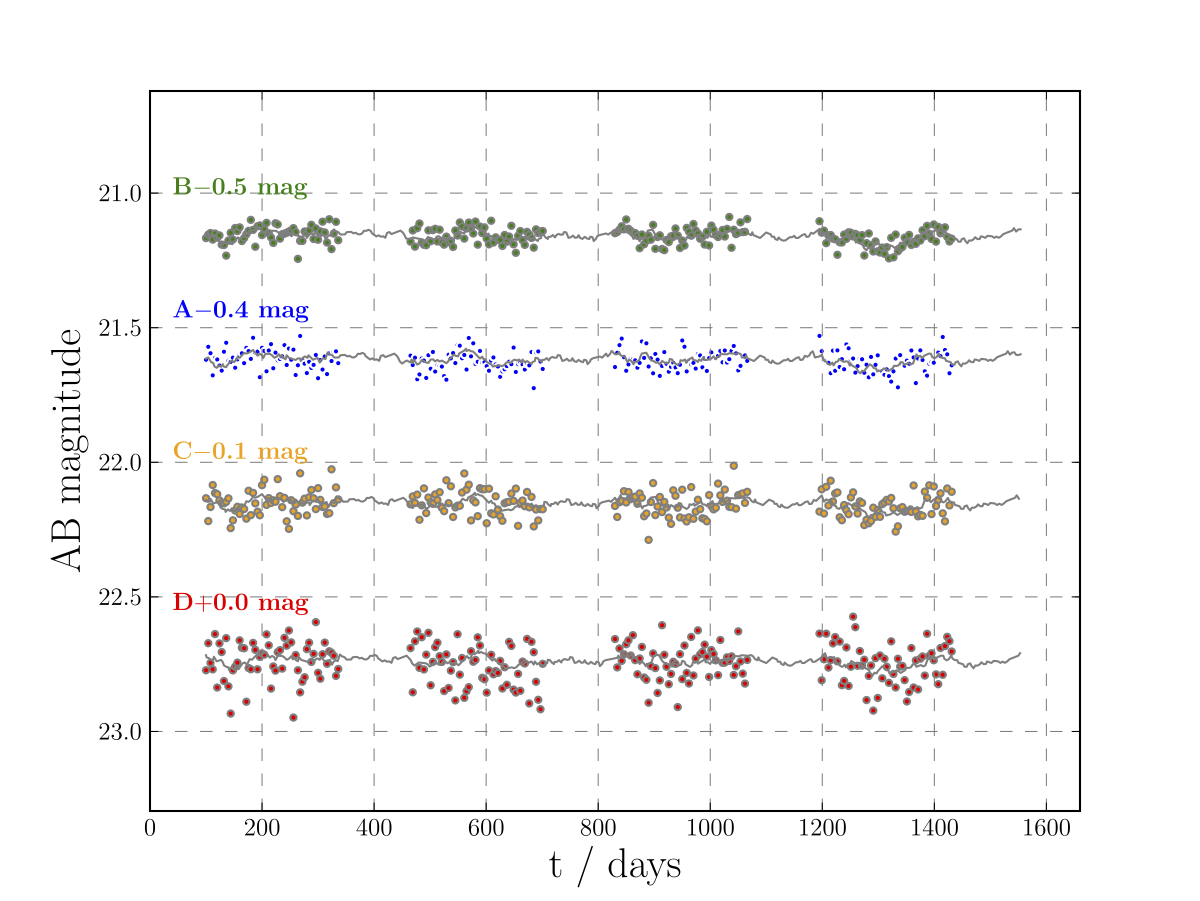
\includegraphics[width=\linewidth]{figs1/oguri_qso_ID=3042348_tau=31_sigma=4_cadence=4_season=8_lightcurve.eps}
\end{minipage}
\begin{minipage}{0.48\linewidth}
\centering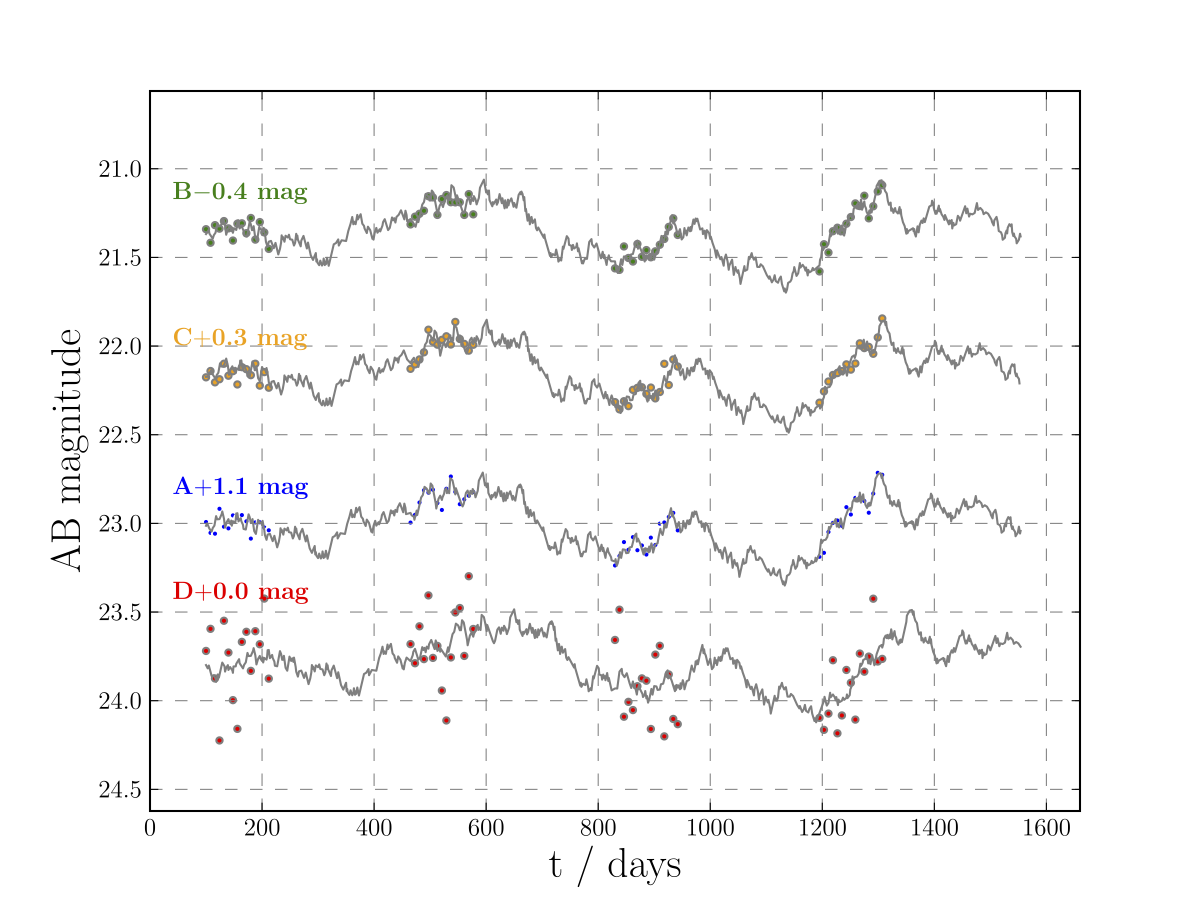
\includegraphics[width=\linewidth]{figs1/oguri_qso_ID=5058554_tau=3162_sigma=16_cadence=8_season=4_lightcurve.eps}
\end{minipage}\hfill
\caption{Two example simulated lensed AGN datasets (with no microlensing).
Left: a minimally-variable source ($\tau_q = 31.62$ days, $\sigma_q = 0.004$),
lensed into a cross configuration (lens ID 3042348), and monitored with high
cadence and long season length (4 days, 8 months, strategy D). Right: a
maaximally-variable source ($\tau_q = 3162$ days, $\sigma_q = 0.016$), lensed
into a major axis cusp configuration (lens ID 5058554), and monitored with low
cadence and short season length (8 days, 4 months, strategy A).
\label{fig:simdata}}
\end{figure*}
%%%%%%%%%%%%%%%%%%%%%%%%%%%%%%%%%%%%%%%%%%%%


\subsubsection{Results}

Strategy B, dt recovery across sample. 3x3x3 = 27 inferences, 27x18 dt estimates. Are
uncertainties on dt accurate? Trends with dt.

Effect of changing observing strategy.

Mean mag and var par recovery across sample. Trends with tau and sigma.



% - - - - - - - - - - - - - - - - - - - - - - - - - - - - - - - - - - - - - - - 

\subsection{Including Microlensing}

In this section we describe our simulations of the microlensing occurring at
each image position, and then repeat the inferences of the previous section in
the presence of this contaminant. How is the time delay inference degraded?
Can the microlensing curves be modelled by the GP? How are the results
affected by observing strategy?


\subsubsection{Methodology}

\TODO{GD}{Write this section please!}
\TODO{PJM/BJB}{Suitable illustrative figure?}

Stellar mass distributions were ``painted on'' to the model lens galaxies, as
described in Dobler et al.\, (in preparation). Established galaxy scaling
relations were used to draw luminosities and effective radii given the model
velocity dispersions; a surface brightness distribution with the same
ellipticity as that of the lens mass, and with a de Vaucoleurs cite profile 
were assumed. Finally, a mass to light ratio was assumed, and the fraction of
surface mass density in the form of stars ($\fstar$) 
computed, at each image position. This parameter, the local lens
convergence, and its shear, were then used to generate a starfield at each
image position, and compute the corresponding source plane magnification map,
using the code of ...

Wambsganss maps. Then, parameters chosen to span the possibilities. Constant
speed traversals, 2 speeds (fast and slow).  2 source sizes, from Kochanek etc
work, separated by factor of 3 (large and small).  fstar values chosen in
catalog and in lens selection, check they are high (c. 0.5).  Check timescales
compared to length of dataset. Illustrative plot. 

Apply to 3 lenses with "typical" intrinsic variabilities, ie the middle tau
and sigma of the 3x3 grid in the previous section. 

\subsubsection{Results}

dt recovery across sample. 3x(2x2) = 12 inferences, 12x18=216 dt estimates.
Are uncertainties on dt accurate? Trends with dt.

Mean mag and ml par recovery across sample. 48 microlensing lightcurves (4
images times 3 lenses x 4 setups). Trends with fstar, source size and v.

% - - - - - - - - - - - - - - - - - - - - - - - - - - - - - - - - - - - - - - - 

\subsection{Discussion}

What did we learn from simulated data?
When do we succeed and when do we fail?
WHat future work is required?

% -----------------------------------------------------------------------------

\section{Application to B1608$+$656}

B1608$+$656 is a gravitational lens system a radio-loud source galaxy; it has 
very precisely measured time delays, and has been successfully used as a
cosmographic probe \citep[e.g.][]{Suy++10}.  Three seasons of VLA monitoring
were taken by  \citet{2002ApJ...581..823F, 1999ApJ...527..498F},  and are
shown in Figure~\ref{b1608_data}. The dominant effect visible in the data is
the gradual change in the flux of the background AGN over time, visible in all
four images. This gradual change is not so useful for measuring the time
delays. Instead, the time delay information comes mostly from small short-term
fluctuations on top of the global trend. The size of the radio source is
assumed to be much larger than the Einstein radius of the stars in the lens
galaxy, leading to negligible microlensing. In this section we model the
B1608$+$656 radio lightcurve data with our combined intrinsic plus
microlensing Gaussian process, to test this assumption and re-measure the
system time delays.

%%%%%%%%%%%%%%%%%%%%%%%%%%%%%%%%%%%%%%%
\begin{figure*}
\includegraphics[scale=0.75]{figs1/b1608_data.eps}
\caption{Monitoring data for B1608+656.\label{b1608_data}}
\end{figure*}
%%%%%%%%%%%%%%%%%%%%%%%%%%%%%%%%%%%%%%%

%%%%%%%%%%%%%%%%%%%%%%%%%%%%%%%%%%%%%%%
\begin{figure*}
\includegraphics{figs1/b1608_delays.eps}
\caption{Inferred time delays for B1608+656.\label{b1608_delays}}
\end{figure*}
%%%%%%%%%%%%%%%%%%%%%%%%%%%%%%%%%%%%%%%

%%%%%%%%%%%%%%%%%%%%%%%%%%%%%%%%%%%%%%%
\begin{figure}
\includegraphics[scale=0.42]{figs1/correlation.eps}
\caption{Inferred intrinsic QSO variability parameters for B1608+656. This is the only significant correlation in the joint posterior distribution. The data are consistent with a small or large value for the variability amplitude, but if the amplitude is large, then the timescale must also be large so that we have only observed a small portion of the timescale.\label{correlation}}
\end{figure}
%%%%%%%%%%%%%%%%%%%%%%%%%%%%%%%%%%%%%%%

% -----------------------------------------------------------------------------

\section{Application to J1131}

\citep{2006astro.ph..5321M}


% -----------------------------------------------------------------------------

\section{Discussion and Further Work}

Robustness of time delays.

Effect of outliers. Do we deal with them well enough in th ecurrent implementation?

Mean mags. implications for millilensing.

Microlensing pars, good enough? Future: inference of physical microlensing parameters. 
Use of informative priors.

Multi-wavelength extension - colour variability.

GP approximations for speed up in LSST era.


% -----------------------------------------------------------------------------

\section{Conclusions}

\begin{itemize}
\item Microlensing can be approximated as GP
\item Time delays and covariance between them can be robustly estimated
\item B1608
\item J1131
\end{itemize}


% -----------------------------------------------------------------------------

\section{Acknowledgements}
David Hogg, Jo Bovy, Malte Tewes, Matt Auger, Sherry Suyu, Chris Fassnacht, Tommaso Treu, Alicia Berciano Alba
(some may be upgraded to authors)

% -----------------------------------------------------------------------------

\begin{thebibliography}{99} 
\bibitem[\protect\citeauthoryear{Brewer 
\& Stello}{2009}]{2009MNRAS.395.2226B} Brewer B.~J., Stello D., 2009, MNRAS, 395, 2226

\bibitem[{Brewer {et~al.}(2010)Brewer, P\'{a}rtay, \& Cs\'{a}nyi}]{dnest}
Brewer, B., P\'{a}rtay, L., \& Cs\'{a}nyi, G. 2010, Statistics and Computing, doi: 10.1007/s11222-010-9198-8, arXiv: 0912.2380

\bibitem[\protect\citeauthoryear{Eigenbrod et 
al.}{2005}]{2005A&A...436...25E} Eigenbrod A., Courbin F., Vuissoz C., Meylan G., Saha P., Dye S., 2005, A\&A, 436, 25 

\bibitem[\protect\citeauthoryear{Fassnacht et 
al.}{2006}]{2006ApJ...642...30F} Fassnacht C.~D., Gal R.~R., Lubin L.~M., 
McKean J.~P., Squires G.~K., Readhead A.~C.~S., 2006, ApJ, 642, 30 

\bibitem[\protect\citeauthoryear{Fassnacht et 
al.}{2002}]{2002ApJ...581..823F} Fassnacht C.~D., Xanthopoulos E., Koopmans 
L.~V.~E., Rusin D., 2002, ApJ, 581, 823 

\bibitem[\protect\citeauthoryear{Fassnacht et 
al.}{1999}]{1999ApJ...527..498F} Fassnacht C.~D., Pearson T.~J., Readhead 
A.~C.~S., Browne I.~W.~A., Koopmans L.~V.~E., Myers S.~T., Wilkinson P.~N., 
1999, ApJ, 527, 498 

\bibitem[\protect\citeauthoryear{Garsden 
\& Lewis}{2010}]{2010NewA...15..181G} Garsden H., Lewis G.~F., 2010, NewA, 15, 181 

\bibitem[\protect\citeauthoryear{Gibbs \& MacKay}{1997}]{gibbsmackay}
Gibbs, M., Mackay, D., 1997, Efficient implementation of Gaussian processes, Cavendish Lab., Cambridge, U.K., Tech. Rep.

\bibitem[\protect\citeauthoryear{Kelly, Bechtold, 
\& Siemiginowska}{2009}]{2009ApJ...698..895K} Kelly B.~C., Bechtold J., Siemiginowska A., 2009, ApJ, 698, 895 

\bibitem[\protect\citeauthoryear{MacLeod et 
al.}{2010}]{2010ApJ...721.1014M} MacLeod C.~L., et al., 2010, ApJ, 721, 
1014 

\bibitem[\protect\citeauthoryear{Morgan et al.}{2008}]{2008ApJ...676...80M} 
Morgan C.~W., Eyler M.~E., Kochanek C.~S., Morgan N.~D., Falco E.~E., 
Vuissoz C., Courbin F., Meylan G., 2008, ApJ, 676, 80 

\bibitem[\protect\citeauthoryear{Morgan et al.}{2006}]{2006astro.ph..5321M} 
Morgan N.~D., Kochanek C.~S., Falco E.~E., Dai X., 2006, astro, 
arXiv:astro-ph/0605321 

\bibitem[\protect\citeauthoryear{Oguri 
\& Marshall}{2010}]{2010MNRAS.405.2579O} Oguri M., Marshall P.~J., 2010, MNRAS, 405, 2579 

\bibitem[\protect\citeauthoryear{O'Hagan 
\& Forster}{2004}]{2004kats.book.....O} O'Hagan A., Forster J., 2004, Kendall's Advanced Theory of Statistics, Volume 2B: Bayesian Inference, London: Hodder Arnold, 2004

\bibitem[\protect\citeauthoryear{Paraficz 
\& Hjorth}{2010}]{2010ApJ...712.1378P} Paraficz D., Hjorth J., 2010, ApJ, 712, 1378 

\bibitem[\protect\citeauthoryear{Pelt et 
al.}{1996}]{1996A&A...305...97P} Pelt J., Kayser R., Refsdal S., Schramm T., 1996, A\&A, 305, 97 

\bibitem[\protect\citeauthoryear{Rasmussen \& Williams}{2006}]{rasmussen} Rasmussen C., Williams C., Gaussian Processes for Machine Learning, The MIT Press, 2006

\bibitem[\protect\citeauthoryear{Schechter}{2005}]{schechter} 
Schechter P.~L., 2005, IAUS, 225, 281 

\bibitem[\protect\citeauthoryear{Suyu et al.}{2010}]{2010ApJ...711..201S} 
Suyu S.~H., Marshall P.~J., Auger M.~W., Hilbert S., Blandford R.~D., 
Koopmans L.~V.~E., Fassnacht C.~D., Treu T., 2010, ApJ, 711, 201 

\bibitem[\protect\citeauthoryear{Suyu et al.}{2009}]{2009ApJ...691..277S} 
Suyu S.~H., Marshall P.~J., Blandford R.~D., Fassnacht C.~D., Koopmans 
L.~V.~E., McKean J.~P., Treu T., 2009, ApJ, 691, 277 

\bibitem[\protect\citeauthoryear{Vuissoz et 
al.}{2008}]{2008A&A...488..481V} Vuissoz C., et al., 2008, A\&A, 488, 481 

\bibitem[\protect\citeauthoryear{Wambsganss}{1999}]{1999JCoAM.109..353W} 
Wambsganss J., 1999, JCoAM, 109, 353 

\bibitem[\protect\citeauthoryear{Zu, Kochanek, 
\& Peterson}{2011}]{2011ApJ...735...80Z} Zu Y., Kochanek C.~S., Peterson B.~M., 2011, ApJ, 735, 80 
\end{thebibliography}

\end{document}

